\documentclass[12pt, a4paper]{article}
\usepackage{ctex}

\usepackage[margin=1in]{geometry}
\usepackage{
  color,
  clrscode,
  amssymb,
  ntheorem,
  amsmath,
  listings,
  fontspec,
  xcolor,
  supertabular,
  multirow,
  mathtools,
  mathrsfs
}
\definecolor{bgGray}{RGB}{36, 36, 36}
\usepackage[
  colorlinks,
  linkcolor=bgGray,
  anchorcolor=blue,
  citecolor=green
]{hyperref}
\newfontfamily\courier{Courier}

\theoremstyle{margin}
\theorembodyfont{\normalfont}
\newtheorem{thm}{定理}
\newtheorem{cor}[thm]{推论}
\newtheorem{pos}[thm]{命题}
\newtheorem{lemma}[thm]{引理}
\newtheorem{defi}[thm]{定义}
\newtheorem{std}[thm]{标准}
\newtheorem{imp}[thm]{实现}
\newtheorem{alg}[thm]{算法}
\newtheorem{exa}[thm]{例}
\DeclareMathOperator{\sft}{E}
\DeclareMathOperator{\idt}{I}
\newcommand{\pr}{\prime}
\DeclareMathOperator{\spn}{span}
\newcommand{\tr}{^\intercal}
\newcommand{\st}{\text{s.t.}}
\newcommand{\hp}{^\prime}
\newcommand{\ms}{\mathscr}
\newcommand{\mn}{\mathnormal}
\newcommand{\tbf}{\textbf}
\newcommand{\mbf}{\mathbf}
\newcommand{\fl}{\mathnormal{fl}}
\newcommand{\f}{\mathnormal{f}}
\newcommand{\g}{\mathnormal{g}}
\newcommand{\R}{\mathbf{R}}
\newcommand{\Q}{\mathbf{Q}}
\newcommand{\JD}{\textbf{D}}
\newcommand{\rd}{\mathrm{d}}
\newcommand{\str}{^*}
\newcommand{\vep}{\varepsilon}
\newcommand{\lhs}{\text{L.H.S}}
\newcommand{\rhs}{\text{R.H.S}}
\newcommand{\con}{\text{Const}}
\newcommand{\oneton}{1,\,2,\,\dots,\,n}
\newcommand{\aoneton}{a_1a_2\dots a_n}
\newcommand{\xoneton}{x_1,\,x_2,\,\dots,\,x_n}
\newcommand\thmref[1]{定理\ref{#1}}
\newcommand\lemmaref[1]{引理\ref{#1}}
\newcommand\defref[1]{定义\ref{#1}}
\newcommand\equref[1]{(\ref{#1})}
\newcommand\figref[1]{图 \ref{#1}}
\newcommand{\remark}{\paragraph{评注}}
\newcommand{\example}{\paragraph{例}}
\newcommand{\proof}{\paragraph{证明}}

\title{科学计算 笔记}
\author{任云玮}
\date{}

\begin{document}
\lstset{numbers=left,
  basicstyle=\scriptsize\courier,
  numberstyle=\tiny\courier\color{red!89!green!36!blue!36},
  language=C++,
  breaklines=true,
  keywordstyle=\color{blue!70},commentstyle=\color{red!50!green!50!blue!50},
  morekeywords={},
  stringstyle=\color{purple},
  frame=shadowbox,
  rulesepcolor=\color{red!20!green!20!blue!20}
}
\maketitle
\tableofcontents
\newpage

\section{绪论}

\subsection{计算机数值计算基本原理}

\subsubsection{实数的存贮方法}
  \begin{defi}[二进制浮点数系]\footnote{floating Number System}
    实数在计算机内部为\tbf{近似存贮},采用二进制浮点数系
    \[
      F(2,n,L,U)=\{\pm0.\aoneton\times10^m\}\cup\{0\}
    \]
    其中$a_1=1$,$a_i\in\{0,\,1\}$. 指数$m$满足$L\le m\le U$.
    称$n$为其字长,$2$表示采用二进制.
  \end{defi}

  \begin{std}[IEEE]
    $\,$
    \begin{enumerate}
      \item 单精度: $t=24,L=-126,U=127$
      \item 双精度: $t=53,L=-1022,U=1023$
      \item Underflow Limit: $UFL=0.1\times2^L$.
      若$0<x<UFL$,则$\\fl(x)=0$.
      \item Overflow Limit: $OFL=0.11\dots1*2^U$.
      若$x>OFL$,则$\fl(x)=\infty$.
      \item 舍入: 若$UFL\le x\le OFL$,则$\fl(x)$为舍入所得浮点数.
      舍入规则如下:设$x=0.\aoneton\dots\times2^m$. 若$a_{n+1}=1$,
      则$d_t+1$并舍弃其后项;否则直接舍弃其后项.
    \end{enumerate}
  \end{std}

  \begin{defi}[机器精度]
    下仅考虑舍去的情况.
    \[\begin{split}
    x-\fl(x) &= 2^m \times 0.0\dots0a_{n+2}\dots \\
    &=2^m \times [2^{-(t+2)} + 2^{-(t+3)} + \cdots] \\
    &=2^m\times2^{-(t+1)}
    \end{split}\]
    其相对误差满足
    \[
      \frac{x-\fl(x)}{x} < \frac{x-\fl(x)}{0.5\times2^m}=2^{-t}
    \]
    记为$\varepsilon$,称之为机器精度.
  \end{defi}

  \begin{pos}
    \[
      \fl(x)=x(1+\delta),\,\text{其中}\,|\delta|\le\varepsilon
    \]
  \end{pos}

\subsubsection{实数的基本运算原理}
  加法$+$硬件实现$\Rightarrow$四则运算.

  \begin{imp}[$x+y$]
    设$x,\,y$为浮点数,则$x+y$的实现方式如下:
    \begin{enumerate}
      \item 对阶:将指数$m$化为两者中较大者;
      \item 尾数相加;
      \item 舍入;
      \item 溢出分析等……
      \item 结果输出.
    \end{enumerate}
  \end{imp}
  \remark
    由$\fl(x)+\fl(y)=x(1+\delta_x)+y(1+\delta_y)$可知,当一个
    大数与一个小数相加时,小数有可能被忽略,所以应当避免大数小数间的相加.

\newpage
\subsection{误差的来源与估计}

\subsubsection{误差的来源}
 \begin{enumerate}
  \item 模型问题. 例:近似地球为球体来计算.
  \item 测量误差. 例:测量地球半径时的误差.
  \item 方法误差(截断误差).
  例:对于$y=\f(x)$,求$\f(x^*)$时使用Taylor展开.
  \item 舍入误差(rounding-off). 例:计算机计算时的误差.
 \end{enumerate}

\subsubsection{误差与有效数字}
  \begin{defi}[绝对误差]
    设$x$为给定实数,$x^*$为其近似值. 定义绝对误差为
    \[
      e(x^*) = x^* - x.
    \]
    称$\varepsilon^*$为其误差上界,若
    \[
      |e(x^*)| \le \varepsilon^*
    \]
  \end{defi}

  \begin{defi}[相对误差]
    对于同上的$x$和$x^*$,定义其相对误差
    \[
      e_r(x^*)=\frac{x^* - x}{x}
    \]
    称$\varepsilon_r^*$为其相对误差界,若
    \[
      |e_r(x^*)|\le\varepsilon_r^*
    \]
  \end{defi}
  \remark
    在实际应用中,$x$通常是未知的,所以会采用
    \[
      \bar{e}_r(x^*)=\frac{x^*-x}{x^*}
    \]
    来代替相对误差. 对于分子,使用绝对误差界来替代,有如下不等式
    \[
      |\bar{e}_r(x^*)| \le \frac{\varepsilon^*}{|x^*|}.
    \]
    这两种相对误差界间的差别,当$\varepsilon^*\ll 1$时,满足
    \[
      |e_r-\bar{e}_r|=O((\varepsilon_r^*)^2)
    \]

  \begin{defi}[有效数字]
    设$x\in R$,$x^*=0.a_1a_2\cdots a_k\times 10^m$为其近似值.
    称$x^*$相对于$x$有$n\,(n\le k)$位有效数字,
    若$n$是满足下式的$n$的最大值.
    \[
      |x^* - x| \le \frac{1}{2} \times 10^{m - n}
    \]
  \end{defi}
  \remark
    在实践中,一般可以采用更加简便的方法,对于归一化以后的$x^*$,
    在尾数部分有$n$位,则称其有$n$位有效数字. 注意,此方法对于
    错误的舍入结果是不适用的,对于错误的情况,需要再减去一位有效
    数字.

  \begin{thm}[误差与有效数字]
    若$x=0.\aoneton\times10^m$有$n$位有效数字,则
    \[
      \vep^*_r \le
      \frac{1}{2a_1}\times10^{1-n}.
    \]
    反之,若
    \[
      \vep^*_r \le
      \frac{1}{2(1+a_1)}\times 10^{1-n},
    \]
    则$x^*$至少有$n$位有效数字.
  \end{thm}
  \proof
    对于前者,只需利用有效数字的定义,以及利用$x\ge 0.a_1$
    (仅考虑$a_1\ne0$的情况). 对于后者,证明是类似的.

\subsubsection{数值运算的误差估计}
  以下内容都假设运算无误差.
  \begin{thm}[四则运算误差估计]
    $\,$
    \begin{enumerate}
      \item 加/减法: $\varepsilon(x\str\pm y\str)
      \le \varepsilon_x\str + \varepsilon_y\str$
      \item 乘法: $\vep(x\str y\str) \le
      |x\str|\vep\str_y + |y\str|\vep\str_x$
      \item 除法: $\vep(\dfrac{x\str}{y\str}) \le
      \dfrac{|x\str|\vep\str_y + |y\str|\vep\str_x}{|y\str|^2}$
    \end{enumerate}
  \end{thm}
  \proof
    考虑加法的误差估计. 对于$x$,$y$及其近似值$x^*$,$y^*$,
    计算$x\str\pm y\str$和$x\pm y$间的误差.
    \[\begin{split}
        & |x\str\pm y\str - ( x \pm y)|
        \le |x\str - x| + |y\str - y|
        \le \varepsilon_x\str + \varepsilon_y\str \\
        \Rightarrow\quad& \varepsilon(x\str\pm y\str)
        \le \varepsilon_x\str + \varepsilon_y\str
    \end{split}\]
    对于其他的运算,证明是类似的. (证明中可用$+1-1$技巧)

  \begin{thm}[运算的误差估计]
    设$A = \f(\tbf{x}) = \f(\xoneton)$,$\tbf{x}\str$是
    $\tbf{x}$的估计值. 利用带Peano余项的Taylor展开,可知
    $A$的绝对误差满足
    \[\begin{split}
      e(A\str) &= \f(\tbf{x}\str) - \f(\tbf{x}) \\
      &= \sum_{p=1}^q\rd^k\f(\tbf{x}\str) + o(||x\str-x||^q) \\
      &\text{取q=1,则} \\
      &= \sum_{k=1}^n\partial_k\f(\tbf{x}\str)(x\str-x) + o(||x\str-x||)
    \end{split}\]
    利用上式,可知
    \[\begin{split}
      &\vep(A\str) \approx
      \sum_{k=1}^n
      \left|\partial_k\f(\tbf{x}\str)\right|\vep(x\str)\\
      &\vep_r(A\str) = \frac{\vep(A\str)}{|A\str|}
    \end{split}\]
  \end{thm}
  \remark
    对于定义在$\R$上的函数,即为
    \[
      \vep(\f(x^*)) \approx |\f\hp(x^*)|\vep(x^*)
    \]

\subsubsection{数字求和的舍入误差分析}
  \begin{pos}
    $n$个浮点数相加,若将它们从小到大排列后相加,则可以减小
    舍入误差.
  \end{pos}
  \proof
    考虑浮点数的求和$S_n=\sum_i^n a_i$,在计算机中的过程表现为
    \[\begin{split}
      & S_2^* = \fl(a_1+a_2)=(a_1+a_2)(1+\vep_2),\quad|\vep_2|\le\vep=2^{-t}\\
      & \cdots\cdots\\
      & S_n^* = \fl(S_{n-1}^*+a_n)(1+\vep_n),\quad|\vep_n|\le\vep
    \end{split}\]
    对于$S_n\str$的误差,若定义$\vep_1=0$,则
    \[
      S_n\str=\sum_{k=1}^n a_k\prod_{p=k}^n(1+\vep_p)
    \]
    对误差进行估计,舍去高阶无穷小,有
    \[
      \prod_{i=k}^n(1+\vep_k)\approx1+\sum_{i=k}^n\vep_k
    \]
    综合上两式,有
    \[\begin{split}
      S_n\str & \approx\sum_{k=1}^na_k(1+\sum_{p=k}^n\vep_p)\\
      & = S_n + \sum_{k=1}^na_k\sum_{p=k}^n\vep_p
    \end{split}\]
    进行移项,并取绝对值,再利用三角不等式,以及$|\vep_i|\le\vep$,得
    \[
      \left|S_n\str-S_n\right|
      \le \sum_{k=1}^n|a_k|\sum_{p=k}^n|\vep_p|
      \le \vep\sum_{k=1}^n|a_k|(n-k+1)
    \]
    其中$n-k+1$关于$k$单调减少,所以根据排序不等式
    [\lemmaref{lemma: 排序不等式}],即可知命题成立. $\blacksquare$

\newpage
\subsection{避免算法失效的基本原则}
  \begin{thm}[原则]
    $\,$
    \begin{enumerate}
      \item 避免两数相除/相减,否则会严重损失有效数字.
      \item 避免两相近数相减.
      \item 避免绝对值很小的数做除数.
      \item 避免大数与小数相加;
      \item 简化计算步骤.
    \end{enumerate}
  \end{thm}


  \begin{alg}[高效计算$e^A$]
    高效计算$e^A$,其中$A\in\R^{n\times n}$. 首先有
    \[
      e^A = e^{(A/2^n)2^n} = B^{2^n}
    \]
    只需要得到$B$,即可以利用倍乘的方法快速得到$B^{2^n}$.
    下对于$B$进行估计. 当$x\to0$时,$e^x$有Taylor展开
    \[
      e^x = 1 + x + \cdots + \frac{x^n}{n!} + \cdots
    \]
    而取足够大的$n$,即可以使得$A/2^n\approx0$,则可以对它
    展开得
    \[
      B \approx I + C + \frac{1}{2}C^2,\,\text{其中}
      C = A/2^n
    \]
    而对于倍乘,考虑$B^2$,展开平方得
    \[
      B^2 \approx I + 2(C+\frac{1}{2}C^2) + (C+\frac{1}{2}C^2)^2
    \]
    从右至左相加即可.
  \end{alg}

  \begin{alg}[秦九韶,多项式估值]
    设有多项式\equref{equ: 多项式},计算$p(z), z\in\R$的值.
    \begin{equation}
      \label{equ: 多项式}
      p(x) = a_0x^n + a_1x^{n-1} + \cdots + a_{n-1}x + a_n
    \end{equation}
    定义$b_n$满足
    \[
      b_0 = a_0, \quad b_k = a_k + b_{k-1}z
    \]
    则$b_n$即为所要求的值. 并且成立
    \[
      p^{\prime}(z) = \sum_{k=0}^{n-1}b_kz^{n-1-k}
    \]
  \end{alg}
  \proof
    用$x-z$去除$p(x)$,记所得余数为$b_n(x)$,即
    \[
      p(x) = (x-z)q(x) + b_n(x),
    \]
    代入$x=z$,则左侧第一项为$0$,可知$p(z) = b_n(z)$.
    将两边的式子展开,利用对应系数相等,即可得算法中$b_n$
    的递推式.

  \begin{thm}[外推法]
    设$x_0$,$x_1$是$x$的两个估计值,且$x_1$相较于$x_0$更
    接近$x$,则可以通过恰当的权值$\omega$,使得它们的加权平均
    \[
      \bar{x} = x_1 + \omega(x_1-x_0)
    \]
    更加接近精确值$x$.
  \end{thm}

  \begin{alg}[$\pi$的估计]
    考虑单位圆,其面积为$\pi$,设$\pi_n$为单位圆的内接正$2n$边形
    的面积,以及
    \[
      \widetilde{\pi}_n = \frac{1}{3}(4\pi_{2n}-\pi_n)
    \]
    则$\pi_n$与$\widetilde{\pi}_n$与$\pi$的误差满足
    \[
      |\pi_n - \pi| = O(\frac{1}{n^2}), \quad
      |\widetilde{\pi}_n - \pi| = O(\frac{1}{n^4})
    \]
  \end{alg}
  \proof
    对于$\pi_n$.
    \[
      \pi_n=n\sin\frac{\pi}{n} =
      \pi - \frac{\pi^3}{3!}\frac{1}{n^2} +
      \frac{\pi^5}{5!}\frac{1}{n^4} - \cdots
      \,\Rightarrow \, |\pi_n - \pi| = O(\frac{1}{n^2})
    \]
    对于$\widetilde{\pi}_n$.
    \[\begin{split}
      \widetilde{\pi}_n & = \pi_{2n} + k(\pi_{2n} - \pi_n)
      = (1+k)\pi_{2n} - k\pi_n \\
      & = (1+k)(\pi - \frac{\pi^3}{3!}\frac{1}{4n^2} + \cdots)
      - k(\pi - \frac{\pi^3}{3!}\frac{1}{n^2} + \cdots) \\
      & = \pi - (\frac{k+1}{4} - k)\frac{\pi^3}{3!}\frac{1}{n^2}
      + O(\frac{1}{n^4})
    \end{split}\]
    为使式子的第二项为零,取$k=\frac{1}{3}$,则成立
    \[
      |\widetilde{\pi}_n - \pi| = O(\frac{1}{n^4})
      \quad\blacksquare
    \]
  \remark
    在实际中,$\pi_n$也是没有办法直接计算而得的,但是对于$n=3$,
    即$6$边形的情况,可以知道$\pi_3=3\sqrt{3}/2$. 同时有递推
    公式
    \[
      \pi_{2n} = \sqrt{2n(n-\sqrt{n^2-\pi^2_n})},
    \]
    而开平方可以通过迭代的方式实现,从而即计算得到足够精确的
    $\pi_{2n}$和$\pi_n$.

\newpage
\section{函数的多项式插值}
\subsection{问题的提出}
  \begin{defi}[插值]
    \label{defi: 插值}
    设函数$y = \f(x)$在$[a, b]$上有定义,且已知在点
    $a\le x_0 < x_1 < \cdots < x_n \le b$处的函数值
    $y_i = \f(x_i)$,若存在一简单函数$P(x)$,成立
    \[
      P(x_i) = y_i,
    \]
    则称$P(x)$为$\f(x)$的插值函数,点$x_1,\,x_2,\,\dots,\,x_n$
    称为插值节点,$[a, b]$称为插值区间,求$P(x)$的方法被称为插值法. \par
    若$P(x) \in P_n$为次数不超过$n$的多项式,则称为多项式插值.
  \end{defi}

  \begin{thm}[唯一性]
    给定满足\defref{defi: 插值}的$n+1$个点上的函数值,则
    次数不超过$n$的插值多项式$P_n(x)$存在且唯一.
  \end{thm}
  \proof
    利用待定系数法,设多项式的系数为$a_0,\,\dots\,a_n$,则
    有线性方程组
    \[
      \left\{
      \begin{gathered}
          a_0 + a_1x_0 + \cdots + a_nx_0^n = y_0,\\
          a_0 + a_1x_1 + \cdots + a_nx_1^n = y_1,\\
          \cdots\cdots \\
          a_0 + a_1x_n + \cdots + a_nx_n^n = y_n,\\
      \end{gathered}
      \right.
    \]
    其系数矩阵为Vandermonde矩阵
    \[
      A =
      \begin{pmatrix}
        1 & x_0 & \cdots & x_0^n \\
        1 & x_1 & \cdots & x_1^n \\
        \vdots & \vdots & & \vdots \\
        1 & x_n & \cdots & x_n^n \\
      \end{pmatrix}
    \]
    根据\defref{defi: 插值}中对于$x_i$的要求,矩阵行列式成立
    \[
      \det A = \prod_{i,j=0,\,i>j}^n (x_i - x_j) \ne 0.
    \]
    所以该方程组有唯一解.
  \remark
    虽然插值多项式是唯一的,但是根据基函数的选取的不同,
    系数是不相同的,所以才需要不同的插值方法.

  \iffalse
    给定一个函数$y = y(x)$在$[a, b]$中的点$x_0<\cdots<x_n$相应的函数值
    $y(x_i)$,设法重构函数$y = y(x)$. \footnote{从系统论的观点出发,
    即:已知映射$K$的一系列输入输出对,如何重构该映射$K$. }\par
    一般情况下解不唯一. 所以设$y = y(x)$位于某一函数内,此时可能存在唯一解.
    例如,设$y(x)\in P_n$,则只需知道$n+1$个点的函数值,即可有唯一解.
      或者设输出$y_i$有测量误差.
      \[
      \widetilde{y}_i = \f(x_i) + \vep_i
      \]
      其中$\vep_i$为误差.
      \[
      y = \f(x) + \vep
      \]
      其中$\vep$正态分布. 根据极大似然估计,等价于最小二乘解,
      (输出最小二乘法)
      \[
      \min_{y\in\pi} \sum_{i=0}^n|y_i - y(x_i)|^2
      \]
      其中$\pi$为某一个函数,有两种情况,
      \begin{enumerate}
      \item $\pi$由物理或化学规律确定;(基于机理建模)
      \item $\pi$由数据决定. (基于数据建模)
      \end{enumerate}
      (求关于权重和阈值的优化问题);(非线性最小二乘解).

    \paragraph{系统论的观点}
  \fi

\subsection{Lagrange插值法}
  \begin{thm}[Lagrange插值法]
    \label{thm: Lagrange插值法}
    定义
    \[\begin{split}
      l_i(x) &= \frac{\prod_{j\ne i}(x - x_j)}{\prod_{j\ne i}(x_i - x_j)} \\
      (L_n\f)(x) &= \sum_{i=0}^ny_il_i(x),
    \end{split}\]
    则$L_n\f$即为$\f$的插值多项式.
  \end{thm}
  \proof
    考虑构造$l_i\in P_n$,满足条件$l_i(x_j) = \delta_{ij}$,这样
    $L_n\f=\sum y_il_i$满足要求. 改写条件为(以$l_0$为例)
    \[\begin{split}
      l_0(x) &= \alpha(x-x_1)\cdots(x-x_n) \\
      l_0(x_0) &= 1
    \end{split}\]
    解得
    \[
      \alpha = \frac{1}{(x_0-x_1)\cdots(x_0-x_n)}\quad\blacksquare
    \]
  \remark
    这样构造插值多项式的动机在于在取定插值节点后,插值实际上相当于
    构造一个从$\mbf{y}=(y_0,\,\dots,\,y_n)\in\R^{n+1}$
    到$y^*(x)\in P_n$的一个映射$\ms{F}$,并且可以证明,
    $\ms{F}$是线性的. 因此成立
    \[
      \ms{F}(\mbf{y}) = \ms{F}(\sum_{i=0}^ny_i\mbf{e}_i)
       = \sum_{i=0}^ny_i\ms{F}(\mbf{e}_i)
       = \sum_{i=0}^ny_i l_i(x).
    \]

  \begin{thm}[Lagrange余项公式]
    设符号含义同\thmref{thm: Lagrange插值法}且$\f$充分光滑,则
    对于每一个固定的$x$成立
    \[
      \f(x) - (L_n\f)(x) =
      \frac{\f^{(n+1)}(\xi)}{(n+1)!}\omega_{n+1}(x)
    \]
    其中$\xi\in(a, b)$且
    \[
      \omega_{n+1}(x) = (x-x_0)\cdots(x-x_n).
    \]
  \end{thm}
  \proof
    固定$x\ne x_i$,定义$R(x)$满足
    \[
      \f(x) - (L_n\f)(x) = R(x)\omega_{n+1}(x).
    \]
    构造辅助函数$\g(t)$
    \[
      \g(t) = \f(t) - (L_n\f)(t) - R(x)\omega_{n+1}(t).
    \]
    根据插值法与$R(x)$的定义,成立
    \[
      \g(x_i) = 0,\quad g(x) = 0,
    \]
    即函数$\g(t)$有$n+2$个零点. 反复应用Rolle定理,可知存在
    $\xi\in(a, b)$,成立$\g^{(n+1)} = 0$,即
    \[\begin{split}
      & \g^{(n+1)}(\xi) = \f^{(n+1)}(\xi) - R(x)(n+1)! = 0 \\
      \Rightarrow\quad& R(x) = \frac{\f^{(n+1)}(\xi)}{(n+1)!}
    \end{split}\]
    结合$R(x)$的定义式即可知命题成立. $\blacksquare$
  \remark
    当已知$\f^{(n+1)}$有界时,可以使用此公式进行估计.

\subsection{Runge现象}
  \begin{thm}
    对于复函数$\f(z)$,如果存在$r_0>\frac32(b-a)$,使得
    $\f(z)$在$B_{r_0}(\frac{a+b}{2})$内解析,则
    $P_n(x) = L_n(x)$在$[a, b]$上一致收敛与$\f(z)$.
    这里$B_{r_0}(\frac{a+b}{2})$为以$\frac{a+b}{2}$为圆心,
    $r_0$为半径的圆.
  \end{thm}

\subsection{Newton插值法}
  \begin{exa}
    $n=2$时问题的求解. \par
    设$y^*(x) = a_0 + a_1(x-x_0) + a_2(x-x_0)(x-x_1)$,
    根据$y^*(x_0) = y_0$,$y^*(x_0) = y_0$,得$a_0 = \f(x_0)$,
    $a_0 + a_1(x_1-x_0) = \f(x_1)$,即
    \[
      a_1 = \frac{\f(x_1)-\f(x_0)}{x_1 - x_0}.
    \]
    可以发现$a_1$为
    割线的斜率. 同理可知
    \[
      a_2 = \frac{\f(x_2)-\f(x_0)-a_1(x_2-x_0)}{(x_2-x_0)(x_2-x_1)}
      = \frac{\dfrac{\f(x_2) - \f(x_0)}{x_2-x_0} - \dfrac{\f(x_1) - \f(x_0)}{x_1-x_0}}{x_2-x_1}
    \]
    为斜率的斜率.
  \end{exa}

  \begin{defi}[差商]
    递归$\f(x)$在$x_{i},\,\dots,\,x_{i+n}$的各阶差商为:
    $\f[x_i] = \f(x_i)$,第$k$阶差商为
    \[
      \f[x_i,\,\dots,\,x_{i+k}] =
      \frac{\f[x_{i+1},\,\dots,\,x_{i+k}] - \f[x_i,\,\dots,\,x_{i+k-1}]}
      {x_{i+k} - x_i}
    \]
  \end{defi}


  \begin{thm}[$n$次Newton插值法]
    \label{thm: Newton插值法}
    $x_0,\dots,x_n$为互异插值点,则函数$\f(x)$满足
    \[\begin{split}
      \f(x) =& \f[x_0] + \f[x_0, x_1](x-x_0) + \f[x_0,x_1,x_2](x-x_0))(x-x_1) + \cdots \\
      & + \f[x_0,\dots,x_n](x-x_0)\cdots(x-x_{n-1}) + R_n(x).
    \end{split}\]
    其中$R_n(x)$为其Newton插值多项式的余项,为
    \[
      R_n(x) = \f[x_0,\dots,x_n,x](x-x_0)\cdots(x-x_n).
    \]
  \end{thm}
  \proof
    根据差商的定义,有
    \[\begin{split}
      \f(x) &= \f[x_0] + \f[x_0, x](x-x_0) \\
      \f[x_0, x] &= \f[x_0, x_1] + \f[x_0, x_1, x](x-x_1) \\
      \cdots & \cdots\cdots \\
      \f[x_0,\dots,x_{n-1}, x] &= \f[x_0,\dots,x_n] +
      \f[x_0,\dots,x_n,x](x-x_n)
    \end{split}\]
    将上述式子反复代入它上面的式子,即得Newton插值公式.
  \remark
    Newton插值法的优点在于,当插值点的个数增加时,无需重新计算原有的系数,
    即Newton插值多项式是可以递归计算的.

  \begin{thm}
    根据Newton插值公式,可以得到如下差商的性质.
    \begin{enumerate}
      \item
      \[
        \f[x_0,\dots,x_m] =
        \sum_{i=0}^m\frac{\f(x_i)}{\prod_{j\ne i}(x_i-x_j)}
      \]
      \item 设$i_0,\dots,i_m$为$0,\dots, m$的任意一个排列,则
      \[
        \f[x_0,\dots,x_m] = \f[x_{i_0},\dots,x_{i_m}].
      \]
      \item 广义Lagrange中值定理
      \[
        \f[x_0,\dots,x_m] = \frac{\f^{(m)}(\xi)}{m!},\quad
        \xi\in(\min\{x_i\}, \max\{x_i\})
      \]
    \end{enumerate}
  \end{thm}
  \proof
    交换插值节点的顺序后,$n$次Newton插值多项式的$n$次项系数不变,
    所以[2.]成立. 同$m-1$次的Lagrange插值多项式比较第$m-1$次
    项系数及其余项,即可得到[1.]和[3.]
  \remark
    根据[3.]可知,对于一个$n$次多项式,$n$阶差商即为其$n$次项系数,
    $k(k>n)$阶差商为零.

  \begin{defi}
    \label{def: 算符}
    给定序列$\{\f_k\}$,$\f_k$表示$\f$在$x=x_k$处的值,定义
    \begin{enumerate}
      \item 前向差分算符$\Delta\f_k = \f_{k+1} - \f_k,$
      \item 移位算符$\sft\f_k = \f_{k+1},$
      \item 恒等算符$\idt\f_k = \f_k.$
    \end{enumerate}
  \end{defi}

  \begin{thm}[算符二项式定理]
    \label{thm: 算符二项式定理}
    对于算符$A$,$B$,若它们可交换,则成立二项式定理
    \[
      (A+B)^m = \sum_{k=0}^m \binom{m}{k} A^kB^{m-k}
    \]
  \end{thm}

  \begin{pos}
    根据\defref{def: 算符}和\thmref{thm: 算符二项式定理}可知
    \[\begin{split}
      \Delta &= \sft - \idt \\
      \Delta^n &= \sum_{k=0}^n\binom{n}{k}(-\idt)^{n-k}\sft^k \\
      \sft^n &= \sum_{k=0}^n\binom{n}{k}\Delta^k
    \end{split}\]
  \end{pos}

  \begin{thm}[均匀插值]
    \label{thm: 均匀插值}
    设$x_0,x_1,\dots,x_n$满足$x_k = x_0 + kh$,则有
    \[\begin{split}
      \f[x_k, x_{k+1}] &= \frac{\Delta\f_k}{h} \\
      \f[x_k, x_{k+1}, x_{k+2}] &=
      \frac{\Delta^2\f_k}{2h^2} \\
      \cdots & \cdots \\
      \f[x_k, \dots,x_{k+m}] &=
      \frac{\Delta^m\f_k}{m!h^m} \\
    \end{split}\]
  \end{thm}

  \begin{thm}[Newton前插公式]
    设记号同\thmref{thm: 均匀插值},另$x = x_0 + th$,$t\in\R$,
    代入\thmref{thm: Newton插值法},则成立
    \[\begin{split}
      N_n(x) =& \f_0 + t\Delta\f_0 + \frac{t(t-1)}{2!}\Delta^2\f_0 + \cdots + \frac{t(t-1)\cdots(t-n+1)}{n!}\Delta^n\f_0.
    \end{split}\]
    其余项为
    \[
      R_n(x) = \frac{t(t-1)\cdots(t-n)}{(n+1)!}h^{n+1}\f^{(n+1)}(\xi),
      \quad \xi\in(x_0, x_n)
    \]
  \end{thm}
  \remark
    利用广义二项式定理,有
    \[\begin{split}
      \f(x) &= \f(x_0 + th) = \sft^t\f(x_0) = (\idt+\Delta)^t\f(x_0) \\
      &= \sum_{k=0}^\infty\binom{t}{k}\Delta^k\f_0
    \end{split}\]

\subsection{Hermite插值}
  \begin{thm}
    设$\f\in C^n[a,b]$,$x_0,x_1,\dots,x_n$为$[a, b]$上的互异节点,
    则$\f[x_0,\dots,x_n,x]$在$[a, b]$上连续.
  \end{thm}

  \begin{thm}[Hermite插值]
    若给出$m+1$个插值条件(含函数值和导数值)可构造出次数不超过$m$次的
    多项式.
  \end{thm}
  \remark
    可以利用待定系数法或者基函数法求的Hermite插值多项式.

\subsection{分段低次多项式插值}
  \paragraph{思路}
    局部入手,整体分析\footnote{例:微分流形}.
    化整为零,以直代曲\footnote{例:Riemann积分}.

  \begin{lemma}[$\omega_n$的估计]
    任给节点$x_0<x_1<\cdots<x_n$,记$h = \max{x_{i+1}-x_i:
    i=0,1,\dots,n}$,则对于任意$x\in[x_0,x_n]$,成立
    \[
      |(x-x_0)\cdots(x-x_n)| \le \frac{n!h^{n+1}}{4}.
    \]
  \end{lemma}

  \begin{thm}[分段线性插值]
    记$a = x_0 < \cdots x_n = b$,$e_k = (x_k, x_{k+1})$,
    $h_k = x_{k+1} - x_k$,$h = \max h_k$. 找函数$y=\f_h(x)$,
    逼近原有函数,使得
    \begin{enumerate}
      \item 满足插值条件,$\f_h(x_k) = \f(x_k)$,
      \item $\f_h(x)$连续,
      \item $\f_h(x)\in P_1$,$x\in e_k$.
    \end{enumerate}
    则$\f_h$的结果为
    \[
      \f_h(x) = \f_h(x_k) + \f_h[x_k, x_{k+1}](x-x_k),
      \quad(x\in e_k).
    \]
    设$M_2$表示二阶导数的上界,则误差$R(x)$满足,
    \[
      R(x) = \left|\frac{\f^{(2)}(\xi)}{2}(x-x_k)(x-x_{k+1})\right|
      \le \frac{1}{8}M_2h^2.
    \]
  \end{thm}
  \remark
    若作整体的Lagrange插值,则余项$R_L(x)$满足
    \[
      \left|\frac{\f^{(n+1)}(\xi)}{(n+1)!}\omega_{n+1}\right|
      \le \frac{M_{n+1}h^{n+1}}{n+1}.
    \]
    而求高阶导数后容易出现Runge现象.

  \begin{thm}[分段三次Hermite插值]
    节点同上,构造$\f_h(x)$使得
    \begin{enumerate}
      \item $\f_h(x_k) = \f(x_k),\,\f_h\hp(x_k) = \f\hp(x_k)$
      \item $\f\in \ms{C}^1[a, b]$
      \item $\f_n(x) \in P_3,\,x\in e_k$
    \end{enumerate}
    对于两插值点的情况,$\f$的结果为
    \[
      \f_h(x) = \f(x_k)\alpha_k + \f(x_{k+1})\alpha_{k+1}
       + \f\hp(x_k)\beta_k + \f\hp(x_{k+1})\beta_{k+1}.
    \]
    其余项$R(x)$满足
    \[
      R(x) = \left|\frac{\f^{4}(\xi)}{4}(x-x_{k})^2(x-x_{k+1})^2\right|
      \le \frac{M_4}{4!}\times\left(\frac{h}{4}\right)^4
      =\frac{1}{384}M_4h^4.
    \]
  \end{thm}

\subsection{三次样条插值}
  \begin{defi}
    \label{defi: 三次样条插值}
    给定控制点$a = x_0 < \cdots < x_n = b$,设函数$y=y^*(x)$满足
    \begin{enumerate}
      \item $y^*(x) = y_k$,
      \item $(y^*)^{(4)} = 0,x\in e_k\,\Leftrightarrow
      \,y^* \in P_3,x\in e_k$,
      \item $y^*\in\ms{C}^2[a, b]$.
    \end{enumerate}
    称满足后两个条件的函数为\tbf{三次样条函数},称满足上述三个条件的函数
    为\tbf{三次样条插值函数}.
  \end{defi}

  \begin{defi}[边界条件]
    $\,$
    \begin{enumerate}
      \item 转角条件:$S\hp(x_0) = \f_0\hp$,$S\hp(x_n) = \f_n\hp$,
      \item 弯矩条件:$S^{\prime\prime}(x_0) = \f_0^{\prime\prime}$,
      $S^{\prime\prime}(x_n) = \f_n^{\prime\prime}$,称
      $S^{\prime\prime}(x_0) = S^{\prime\prime}(x_n) = 0$的特例为
      自然边界条件,
      \item 周期条件:$S(x_0+0)=S(x_n-0)$,$S\hp(x_0+0)=S\hp(x_n-0)$,
      $S^{\prime\prime}(x_0+0)=S^{\prime\prime}(x_n-0)$,
      \item 非纽结条件:$S^{\pr\pr\pr}(x)$在$x=x_1$和$x=x_{n-1}$处
      连续. \footnote{(Not-a-knot end Condition)这是Matlab中spline在$X$和$Y$长度相同时所应用的边界
      条件. }
    \end{enumerate}
  \end{defi}
  \remark
    根据\defref{defi: 三次样条插值},在每个小区间上有$4$个待定系数,
    所以总共有$4n$个待定系数. 而所给条件仅有$n+1$个插值条件,以及在
    中间$n-1$个插值节点处二阶导数连续(从而原函数与一阶导数也连续),
    有$3n-3$个光滑性条件,共$4n-2$个条件,因此需要额外的边界条件来确定
    剩余两个系数.

  \begin{thm}[样条插值的求解]
    设$S^{\pr\pr}(x_i) = M_i$,通过求解$M_i$来确定插值多项式.
    由于$S(x)\in\ms{C}^2$且在每一段上$S(x)\in P_3$,所以$S^{\pr\pr}(x)$
    是分段的线性函数. 设在每一段上,
    \[
      S^{\pr\pr}(x) = M_j\frac{x_{j+1}-x}{x_{j+1}-x_j}
      + M_{j+1}\frac{x-x_j}{x_{j+1}-x_j}.
    \]
    对$S^{\pr\pr}$积分一次、二次,并分别利用光滑性条件、插值条件,以及
    所给定的边界条件,即可求得$M_i$的值.
  \end{thm}

  \begin{thm}
    设$\f(x)\in\ms{C}^4[a, b]$,则三次样条插值函数$S_3(x)$,
    \[
      \max_{a\le x\le b}\left| \f^{(m)}(x) - S^{(m)}(x) \right|
      \le C_m \max_{a\le x\le b}|\f^{(4)}(x)|h^{4-m},\quad
      m=0,1,2,
    \]
    其中$C_0 = 5/384$,$C_1 = 1/24$,$C_2 = 3/8$.
  \end{thm}

\newpage
\section{函数的多项式逼近}
\subsection{绪论}
  \begin{defi}[逼近]
    对函数$\f$逼近,即找一简单函数$\g$,使得在某种度量的意义下,
    它们之间的误差最小或足够小.
  \end{defi}

  \begin{thm}[Weierstrass]
    对于定义在$[a, b]$上的连续复函数,存在一列复多项式$\{P_n\}$,
    成立
    \[
      \lim_{n\to\infty}P_n = \f,
    \]
    且是一致的. 若$\f$是实函数,则$P_n$的系数也为实数.
  \end{thm}
  \remark
    Stone-Weierstrass定理
    \footnote{
      \tbf{Theorem(Stone) }
      Suppose $\ms{A}$ is a self-adjoint algebra of complex
      continuous functions on a compact set $K$, $\ms{A}$
      separates points on $K$, and $\ms{A}$ vanishes at no
      point of $K$. Then the uniform closure $\ms{B}$ of
      $\ms{A}$ consists of all complex continuous functions
      on $K$. In other words, $\ms{A}$ is dense in $\ms{C}(K)$.
    }
    保证了至少在最大模的意义下,用多项式
    来逼近函数是可能的.

  \begin{defi}[常用范数]
    对于$\R^n$,常用的范数有
    \begin{enumerate}
      \item $\|\tbf{x}\|_\infty = \max_{1\le i\le n}|x_i|$,
      \item $\|\tbf{x}\|_1 = \sum_{i=1}^n|x_i|$,
      \item $\|\tbf{x}\|_2 = (\sum_{i=1}^nx_i^2)^{1/2}$.
    \end{enumerate}
    对于$\ms{C}[a, b]$,常用的范数有
    \begin{enumerate}
      \item $\|\f\|_\infty = \max_{a\le x\le b}|\f(x)|$,
      \item $\|\f\|_1 = \int_a^b|\f(x)|\rd x$,
      \item $\|\f\|_2 = (\int_a^b\f^2(x) \rd x)^{1/2}$.
    \end{enumerate}
  \end{defi}
  \remark
    通常对于内积空间$X$,可以定义范数为
    \[
      \|\tbf{x}\| = \sqrt{(x, x)}.
    \]

  \begin{defi}[权函数]
    \label{defi: 权函数}
    设$[a,b]$为有限或无限区间\footnote{例子中说$\rho=1$是一个
    常用的权函数,但我没有明白,在无限区间的时候[1.]是如何成立的. }
    ,
    非负函数$\rho(x)$称为$[a,b]$上的权
    函数,若满足
    \begin{enumerate}
      \item $\int_a^b\rho(x)x^k\rd x < \infty$,$k=0,1,2,\dots$,
      \item 对任意非负$\g\in\ms{C}[a, b]$,若$\int_a^b\rho(x)\g(x)=0$,
      则$g=0$.
    \end{enumerate}
  \end{defi}
  \remark
    利用权函数,可以定义带权内积和范数.

\newpage
\subsection{最佳平方逼近}
  \begin{defi}[最佳平方逼近]
    \label{defi: 最佳平方逼近}
    给定$\f\in\ms{C}[a, b]$和线性无关的函数列$\varphi_0,\dots,
    \varphi_n\in\ms{C}[a, b]$,定义$S_n=\spn\{\varphi_0,
    \dots,\varphi_n\}$,称$\f^*\in S_n$为最佳平方逼近函数,若
    \[
      \|\f^* - \f\| = \min_{\g\in S_n}\|\f-\g\|_2.
    \]
    即$\f^*$是在$2$-范数的含义下,$S_n$中与$\f$最接近的函数.
  \end{defi}
  \remark
    对于离散的情况
    \footnote{
      实际上我们可以利用Riemann-Stieltjes积分定义内积,
      \[\begin{split}
        & (\f,\g) = \int_a^b \f\rd G, \\
        & G(x) =
        \begin{cases}
          \int_a^b\g\rd x,\quad&\text{$\g$为函数,} \\
          \sum_{i=0}^n\f(x_i)I(x-x_i), &\text{$\g$为离散点}
        \end{cases}
      \end{split}\]
      其中$I(x)$为单位阶跃函数. 可以发现,这两种描述的方式是等价的.
      在这样的描述下,对于离散点的$G$实际上是阶梯函数.
    }
    ,可以描述为:给定$x_0,\dots,x_n$处的函数值
    $\f(x_k)$,求$\f^*$,成立
    \[
      \sum_{i=0}^{n}\rho(x_i)|\f(x_j)-\f^*(x_j)|^2 =
      \min_{\g\in S_n}\sum_{i=0}^{n}\rho(x_i)|\f(x_j)-\g(x_j)|^2
    \]

  \begin{thm}[最佳平方逼近的求解]
    设记号同\defref{defi: 最佳平方逼近},设
    \[
      \g(x) = \sum_{i=0}^na_i\varphi_i(x),
    \]
    则可以定义关于$\tbf{a} = (a_0,\dots,a_n)\tr$的函数
    \[\begin{split}
      I(\tbf{a}) = \|\f-\g\|_2^2 &=
      \left\|\f - \sum_{i=0}^na_i\varphi_i\right\|_2^2
      =  \int_a^b \rho\left( \f-\sum_{i=0}^n a_i\varphi_i \right)^2 \rd x.
    \end{split}\]
    根据定义,$I(\tbf{a})$在$\f^*$处取极值,根据Fermat定理,
    在该点各偏导数为零,通常假设$\f$的条件足够好,极限和积分可以换序,即有
    \[\begin{split}
      \frac{\partial I}{\partial a_j} &=
      \int_a^b \frac{\partial}{\partial a_i}
      \rho\left( \f-\sum_{i=0}^n a_i\varphi_i \right)^2 \rd x\\
      &= -2\int_a^b\rho\left( \f-\sum_{i=0}^n a_i\varphi_i \right)\varphi_j \rd x
      = 0.
    \end{split}\]
    即有线性方程组,
    \begin{equation}\begin{cases}
      \label{equ: 法方程}
      (\varphi_0, \varphi_0)a_0 + (\varphi_0, \varphi_1)a_1 + \cdots + (\varphi_0, \varphi_n)a_n = (\f, \varphi_0) \\
      (\varphi_1, \varphi_0)a_0 + (\varphi_1, \varphi_1)a_1 + \cdots + (\varphi_1, \varphi_n)a_n = (\f, \varphi_1) \\
      \dots\dots\\
      (\varphi_n, \varphi_0)a_0 + (\varphi_n, \varphi_1)a_1 + \cdots + (\varphi_n, \varphi_n)a_n = (\f, \varphi_n)
    \end{cases}\end{equation}
    由于$\{\varphi_k\}$线性无关,所以方程组\equref{equ: 法方程}有唯一解.
    设其解为$\tbf{a}^*$,则最佳平方逼近函数即为
    \[
      \f^* = \sum_{i=0}^na^*_i\varphi_i(x),
    \]
  \end{thm}

  \paragraph{几何描述}
    可以从几何的角度来理解最佳平方逼近. $S_n$是$\{\varphi_k\}$
    张成的空间,而$\f$是$S_n$内或$S_n$外的一个向量,最佳平方逼近
    即找$S_n$中找$\f^*$,使得$\|\f-\f^*\|$最小. 根据几何上的直观,
    $\f-\f^*$应该和$S_n$“垂直”,即与张成$S_n$的向量组中的向量分别
    垂直. 而垂直可以被描述为内积为零. 从而就得到了式\equref{equ: 法方程}.
    (见\figref{fig: 最佳平方逼近几何含义})
    \begin{figure}[htbp]
      \centering
      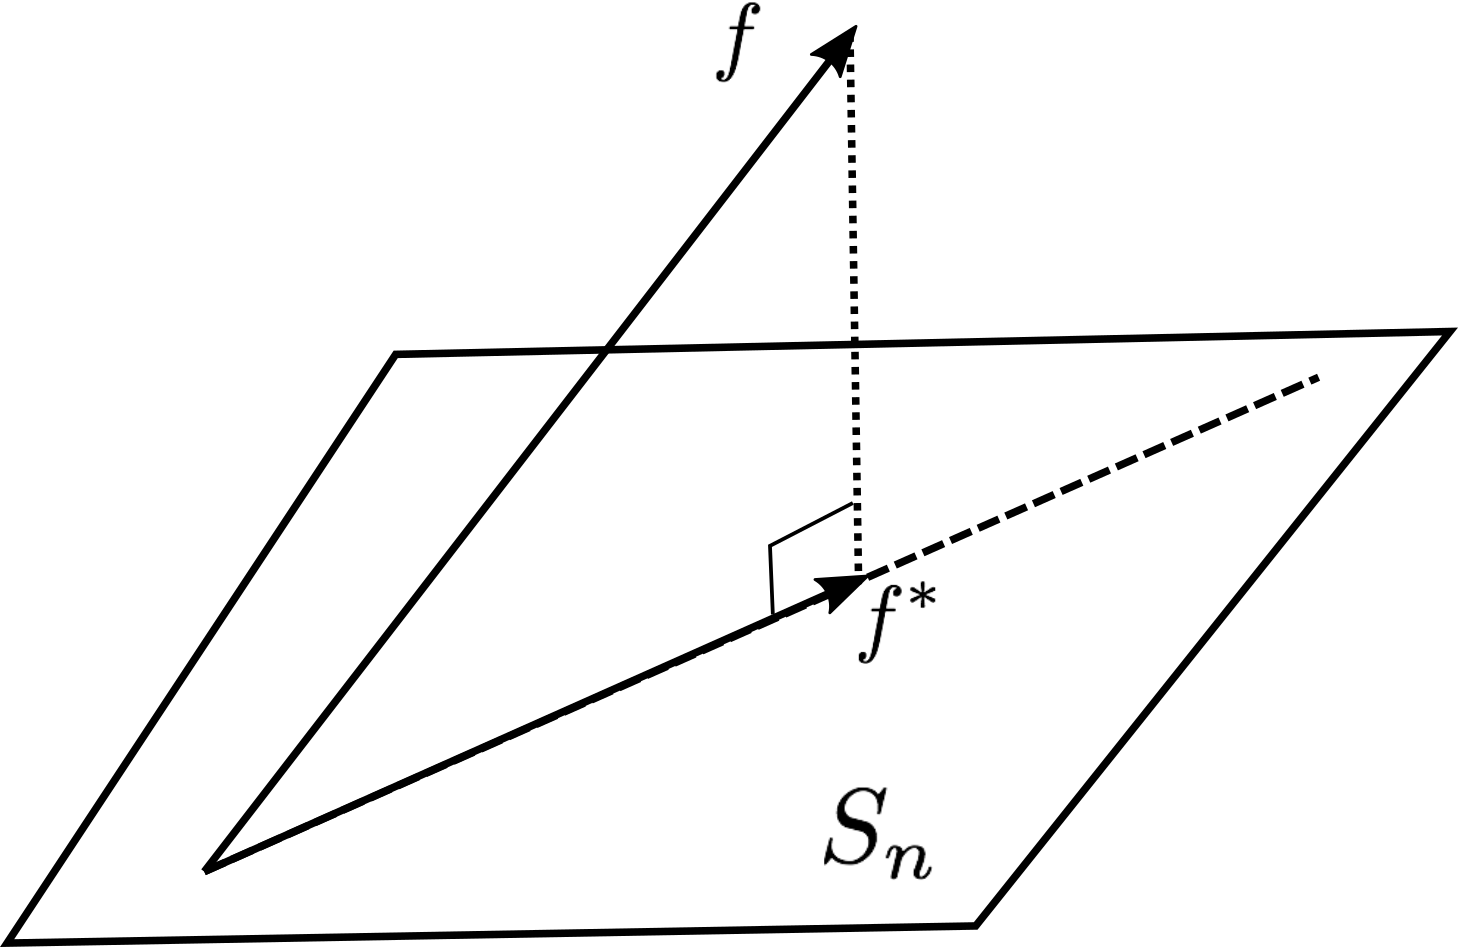
\includegraphics[height=8cm]{../image/least-square.png}
      \caption{最佳平方逼近几何含义}
      \label{fig: 最佳平方逼近几何含义}
    \end{figure}

\newpage
\subsection{正交多项式·绪论}
  \begin{defi}[正交]
    设函数$\f,\g\in\ms{C}[a, b]$,$\rho$为$[a, b]$上的权函数
    且满足
    \[
      (\f, \g) = \int_a^b\rho\f\g\rd x = 0,
    \]
    则称$\f$和$\g$在$[a, b]$上带权$\rho$\tbf{正交}. 若函数组
    $\{\varphi_k\}_{k=0}^\infty$满足
    \[
      (\varphi_i,\varphi_j) =
      \begin{cases}
        0,&\quad i\ne j \\
        A_k>0,& i=j
      \end{cases}
    \]
    则称$\{\varphi_k\}$为$[a, b]$上的带权$\rho$的\tbf{正交函数组}.
    若$A_k=1$,则称为\tbf{标准正交函数组}.
  \end{defi}

  \begin{defi}[正交多项式]
    设$\{\varphi_k\}_{k=0}^\infty$是首项系数$a_n\ne0$的$n$
    次多项式序列. 若它们正交,则称它们为\tbf{正交多项式序列}.
  \end{defi}

  \begin{alg}[Gram-Schmidt正交化]
    设$\{\varphi_k\}$是内积空间$V$的一组基,定义
    \[\begin{split}
      \psi_0 &= \varphi_0, \\
      \psi_{n} &= \varphi_n - \sum_{i=0}^{n-1}(\varphi_i, \eta_i)\eta_i
    \end{split}\]
    其中$\eta_i = \psi_i / \|\psi_i\|$. 则$\{\psi_k\}$为
    $V$的一组正交基.
  \end{alg}
  \remark
    要求$n$次正交多项式组,只需另$\varphi_k = x^k$,再进行
    Gram-Schmidt正交化即可。

  \begin{thm}
    设$\{\varphi_n\}_{n=0}^\infty$是一列正交多项式,
    根据正交性(从而线性无关)可以得到正交多项式的如下性质,
    \begin{enumerate}
      \item $P_n \subset \spn\{\varphi_0, \dots,\varphi_n\}$,
      \item 设$P\in P_{n-1}$,则$\varphi_n$与$P$正交.
    \end{enumerate}
  \end{thm}

  \begin{thm}
    设$\{\varphi_n\}_{n=0}^\infty$是$[a,b]$上带权$\rho$的
    正交多项式,则成立
    \[
      \varphi_{n+1} = (x-\alpha_n)\varphi_n - \beta_n\varphi_{n-1},
      \quad n = 0, 1,\dots,
    \]
    其中
    \[\begin{split}
      &\varphi_0 = 1,\quad \varphi_{-1} = 0,\\
      &\alpha_n = (x\varphi_n, \varphi_n) / (\varphi_n, \varphi_n),\\
      &\beta_n = (\varphi_n, \varphi_n) / (\varphi_{n-1}, \varphi_{n-1}).
    \end{split}\]
  \end{thm}
  \proof
    由于齐次性,不妨设$\varphi_n$首项系数为$1$. 所以成立
    \[
      \varphi_{n+1}-x\varphi_n = \sum_{k=0}^n\gamma_k\varphi_k,
    \]
    对于系数$\gamma_k$,成立
    \footnote{
      设$B$是内积空间$V$的一组正交基,则对于任意
      $x\in V$,成立
      \[
        x = \sum_{\beta\in B}\frac{(x,\beta)}{(\beta,\beta)}\beta
      \]
      另外,根据这里内积的定义,成立$(\varphi_i,\varphi_j)
      =(\varphi_i/x, x\varphi_j)$.
    }
    \[
      \gamma_k = \frac{(\varphi_{n+1}-x\varphi_n,\varphi_k)}
      {(\varphi_k, \varphi_k)}
      = \frac{(\varphi_{n+1},\varphi_k) - (\varphi_n, x\varphi_k)}{(\varphi_k,\varphi_k)}.
    \]
    由于$\{\varphi_n\}$正交,所以当$k<n-1$时,成立$\gamma_k=0$.
    所以有
    \[
      \varphi_{n+1} - x\varphi_n = \gamma_n\varphi_n + \gamma_{n-1}\varphi_{n-1}.
    \]
    再进行一些代换,即可以得到原递推式. $\blacksquare$

  \begin{thm}
    设$\{\varphi_n\}_{n=0}^\infty$为$[a, b]$上带权$\rho$的
    正交多项式,则$\varphi_n$在区间$(a, b)$上有$n$个不同的零点。
  \end{thm}
  \proof
    首先利用权函数的定义,证明零点不可能都是偶数重的。再假设
    $x_1,\dots,x_l$是$\varphi_n$的奇数重零点,则
    \[
      \left(\varphi_n, (x-x_1)\cdots(x-x_l)) \right) \ne 0,
    \]
    再利用正交性可得$l=n$. $\blacksquare$

\newpage
\subsection{Legendre多项式}
  \begin{defi}[Legendre多项式]
    取区间$[-1, 1]$,$\rho(x)\equiv1$,称由$\{1,x,\dots,x^n,\dots\}$
    正交化而得的多项式为Legendre多项式。其表达式为
    \[
      P_0(x) = 1,\quad
      P_n(x) = \frac{1}{2^nn!}\frac{\rd^n}{\rd x^n}(x^2-1)^n,
      \quad n=1,2,\dots
    \]
    首项系数为$1$的Legendre多项式为
    \[
      \widetilde{P}_n(x) = \frac{n!}{(2n)!}\frac{\rd^n}{\rd x^n}(x^2-1)^n.
    \]
  \end{defi}

  \begin{thm}[Legendre多项式的性质]
    Legendre多项式有如下性质,
    \begin{enumerate}
      \item 正交性:
      \[
        \int_{-1}^1 P_n(x)P_m(x)\rd x =
        \begin{cases}
            0, &\quad m\ne n, \\
            \dfrac{2}{2n+1},&\quad m = n.
        \end{cases}
      \]
      \item 奇偶性:
        \[P_n(x) = (-1)^nP_n(-x),\]
      \item 递推关系:
      \[
        (n+1)P_{n+1} = (2n+1)xP_n - nP_{n-1},\quad
        n = 1, 2,\dots
      \]
    \end{enumerate}
  \end{thm}
  \proof todo

  \begin{thm}[Legendre多项式的逼近性质]
    在区间$[-1, 1]$上,设$\widetilde{L}_n$是首项系数为$1$的
    Legendre多项式,则
    \[
      \|\widetilde{L}_n\|_2 = \min_{P\in P_n}\|P(x)\|_2.
    \]
  \end{thm}

\newpage
\subsection{Chebyshev多项式}
  \begin{defi}[Chebyshev多项式]
    取区间$[-1, 1]$,$\rho(x)=(1-x^2)^{-1/2}$,称由$\{1,x,\dots,x^n,\dots\}$
    正交化而得的多项式为Chebyshev多项式。其表达式为
    \[
      T_n(x) = \cos(n\arccos x),\quad|x|\le 1
    \]
  \end{defi}

  \begin{thm}[Chebyshev多项式的性质]
    Chebyshev多项式有如下性质,
    \begin{enumerate}
      \item 递推关系:
      \[\begin{split}
        &T_0(x) = 1, \quad T_1(x) = x,\\
        &T_{n+1}(x) = 2xT_n(x) - T_{n-1}(x),\quad n =1,2,\dots
      \end{split}\]
      \item 正交性:
      \[
        \int_{-1}^1\frac{T_n(x)T_m(x)}{\sqrt{1-x^2}} \rd x =
        \begin{cases}
          0, &\quad n\ne m,\\
          \pi/2, &\quad n = m \ne 0,\\
          \pi,&\quad n = m = 0.
        \end{cases}
      \]
      \item $T_{2k}(x)$只含$x$的偶次幂,$T_{2k+1}(x)$只含$x$的
      奇次幂。
      \item $T_n$在区间$[-1, 1]$上的$n$个零点为
      \[
        x_k = \cos\frac{2k-1}{2n}\pi,\quad k = 1,2,\dots,n.
      \]
      \item $T_n$的首项系数为$2^{n-1}$.
    \end{enumerate}
  \end{thm}

  \begin{thm}[Chebyshev多项式的逼近性质]
    \label{thm: Chebyshev多项式的逼近性质}
    在区间$[-1,1]$上,设$\widetilde{T}_n$是首项系数
    为$1$的Chebyshev多项式,则
    \[
      \|\widetilde{T}_n\|_\infty = \min_{P\in\widetilde{P}_n}
      \|P(x)\|_\infty = \frac{1}{2^{n-1}}.
    \]
  \end{thm}
  \remark
    这一定理意味着,取区间$[-1, 1]$,$n$次Chebyshev多项式是所有次数
    小于等于$n$的首项为$1$的多项式中,绝对值的最大值最小的一个。从而,
    若想用$P_{n-1}$中的多项式来逼近$n$次多项式$\f$,只需找
    $\f^*\in P_{n-1}$,使得
    \[
      \f - \f^* = a_n \widetilde{T}_n.
    \]
    其中$a_n$为$\f$的$n$次项系数。对于一般的在区间$[a, b]$上的情况,
    只需利用平移和伸缩映射到$[-1, 1]$上即可。

  \begin{thm}[Chebyshev零点插值]
    设插值节点$x_0,\dots,x_n$为Chebyshev多项式$T_{n+1}$的
    零点,被插值函数$\f\in\ms{C}^{n+1}[-1, 1]$,则多项式插值
    的余项$R_n$满足
    \[
      |R_n| \le \frac{1}{2^n(n+1)!}\|\f^{(n+1)}(x)\|_{\infty}.
    \]
  \end{thm}
  \proof
    由于插值点是Chebyshev多项式的零点,所以$\omega_{n+1}=
    \widetilde{T}_n$,所以根据\thmref{thm: Chebyshev多项式的逼近性质},成立
    \[
      \omega_{n+1} \le \frac{1}{2^n}.\quad\blacksquare
    \]
  \remark
    这一定理保证了使用Chebyshev多项式的零点插值,至少可以使得
    误差的最大值最小。

\newpage
\section{附录}
\subsection{不等式}

  \begin{lemma}[排序不等式]
    \label{lemma: 排序不等式}
    对于满足下述条件的$\{a_n\}$,$\{b_n\}$,
    \[\begin{split}
      & 0 \le a_1\le a_2\le\cdots\le a_n \\
      & 0 \le b_1\le b_2\le\cdots\le b_n
    \end{split}\]
    则同序相乘求和值最大,逆序最小,即
    \[
      \sum_{i=1}^n a_ib_i \ge \sum_{i=1}^n a_ib_{k_i}
      \ge \sum_{i=1}^n a_ib_{n-i+1}
    \]
  \end{lemma}

  \begin{lemma}[算数-几何均值不等式]
    \[
      (a_1a_2\cdots a_n)^{1/n} \le \frac{a_1+a_2+\cdots+a_n}{n}
    \]
    当且仅当$a_1 = a_2 = \cdots = a_n$时等号成立.
  \end{lemma}
  \proof
    因为有齐次性,所以不妨设$\prod a_i=1$,并令
    \[
      a_1=\frac{\alpha_1}{\alpha_2},\quad
      \dots,\quad
      a_{n-1} = \frac{\alpha_{n-1}}{\alpha_n},\quad
      a_n = \frac{\alpha_n}{\alpha_1}
    \]
    则只需证明下式即可.
    \[
      \frac{\alpha_1}{\alpha_2} + \cdots + \frac{\alpha_n}{\alpha_1}
      \ge n
    \]
    不妨设$\alpha_1 \le \alpha_2 \le \cdots \le \alpha_n$,则根据排序不等式
    \[
      \lhs \ge \alpha_1\frac{1}{\alpha_1} + \cdots + \alpha_n\frac{1}{\alpha_n}
       = n \quad\blacksquare
    \]

\end{document}
